\documentclass[aip,jcp,reprint,noshowkeys,superscriptaddress]{revtex4-1}
\usepackage{graphicx,dcolumn,bm,xcolor,microtype,multirow,amscd,amsmath,amssymb,amsfonts,physics,longtable,wrapfig}
\usepackage[version=4]{mhchem}

\usepackage[utf8]{inputenc}
\usepackage[T1]{fontenc}
\usepackage{txfonts}

\usepackage[
    colorlinks,
    linkcolor={red!50!black},
    citecolor={red!70!black},
    urlcolor={red!80!black}
	]{hyperref}
\urlstyle{same}

\newcommand{\ie}{\textit{i.e.}}
\newcommand{\eg}{\textit{e.g.}}
\newcommand{\alert}[1]{\textcolor{red}{#1}}
\usepackage[normalem]{ulem}
\newcommand{\titou}[1]{\textcolor{red}{#1}}
\newcommand{\trashPFL}[1]{\textcolor{\red}{\sout{#1}}}
\newcommand{\PFL}[1]{\titou{(\underline{\bf PFL}: #1)}}

\newcommand{\cre}[1]{\Hat{a}_{#1}^{\dag}}
\newcommand{\ani}[1]{\Hat{a}_{#1}}
\newcommand{\ca}[2]{\Hat{a}^{#1}_{#2}}

\newcommand{\mc}{\multicolumn}
\newcommand{\fnm}{\footnotemark}
\newcommand{\fnt}{\footnotetext}
\newcommand{\tabc}[1]{\multicolumn{1}{c}{#1}}
\newcommand{\QP}{\textsc{quantum package}}
\newcommand{\T}[1]{#1^{\intercal}}

% coordinates
\newcommand{\br}{\boldsymbol{r}}
\newcommand{\bx}{\boldsymbol{x}}
\newcommand{\bI}{\boldsymbol{1}}
\newcommand{\cK}{\mathcal{K}}

% orbital energies
\newcommand{\eps}{\epsilon}
\newcommand{\irr}{\text{irr}}

% shortcuts for greek letters
\newcommand{\si}{\sigma}
\newcommand{\la}{\lambda}
\newcommand{\ii}{\mathrm{i}}
\newcommand{\up}{\uparrow}
\newcommand{\dw}{\downarrow}
\newcommand{\upup}{\up\up}
\newcommand{\updw}{\up\dw}
\newcommand{\dwup}{\dw\up}
\newcommand{\dwdw}{\dw\downarrow}

\newcommand{\h}{\text{1h}}
\newcommand{\p}{\text{1p}}
\newcommand{\hp}{\text{1h+1p}}
\newcommand{\hhp}{\text{2h1p}}
\newcommand{\pph}{\text{2p1h}}
\newcommand{\ph}{\text{ph}}
\newcommand{\eh}{\text{eh}}
\newcommand{\he}{\text{he}}
\newcommand{\ee}{\text{ee}}
\newcommand{\teh}{\overline{\text{eh}}}
\newcommand{\pp}{\text{pp}}
\newcommand{\hh}{\text{hh}}
\newcommand{\xc}{\text{xc}}
\newcommand{\Hx}{\text{Hx}}


% addresses
\newcommand{\LCPQ}{Laboratoire de Chimie et Physique Quantiques (UMR 5626), Universit\'e de Toulouse, CNRS, UPS, France}

\begin{document}	

\title{From Parquet to Hedin's Equations}

\author{Pierre-Fran\c{c}ois \surname{Loos}}
	\email{loos@irsamc.ups-tlse.fr}
	\affiliation{\LCPQ}

\begin{abstract}
Hedin's and parquet equations provide two formally exact but apparently
rather different organizations of many-body perturbation theory.
Hedin's equations are formulated in terms of a self-energy, a screened
interaction, and a 3-point vertex, whereas parquet theory resolves the
full 4-point vertex into contributions associated with the three
two-particle scattering channels.
In these notes, we examine explicitly the connection between these two
formulations.
We show that combining the $\eh$ Bethe--Salpeter equation of parquet theory
with the relation between the full vertex and the electron-hole response
yields directly the 4-point Hedin response equation.
The corresponding Hedin kernel is therefore the electron-hole irreducible
parquet vertex,
$
	\fdv*{\Sigma}{G}
	=
	\Gamma^\eh
	=
	\Lambda
	+
	\Phi^{\teh}
	+
	\Phi^\pp
$.
This identity provides a simple interpretation of the relation between the
two theories: parquet keeps the different scattering channels explicit,
whereas the 4-point Hedin formulation combines the transverse
electron-hole and particle-particle channels into a single three-frequency
kernel.
The analogous construction in the particle-particle channel is also briefly
discussed, providing a direct connection with particle-particle Hedin
equations and the $T$-matrix approximation.
\bigskip
\begin{center}
	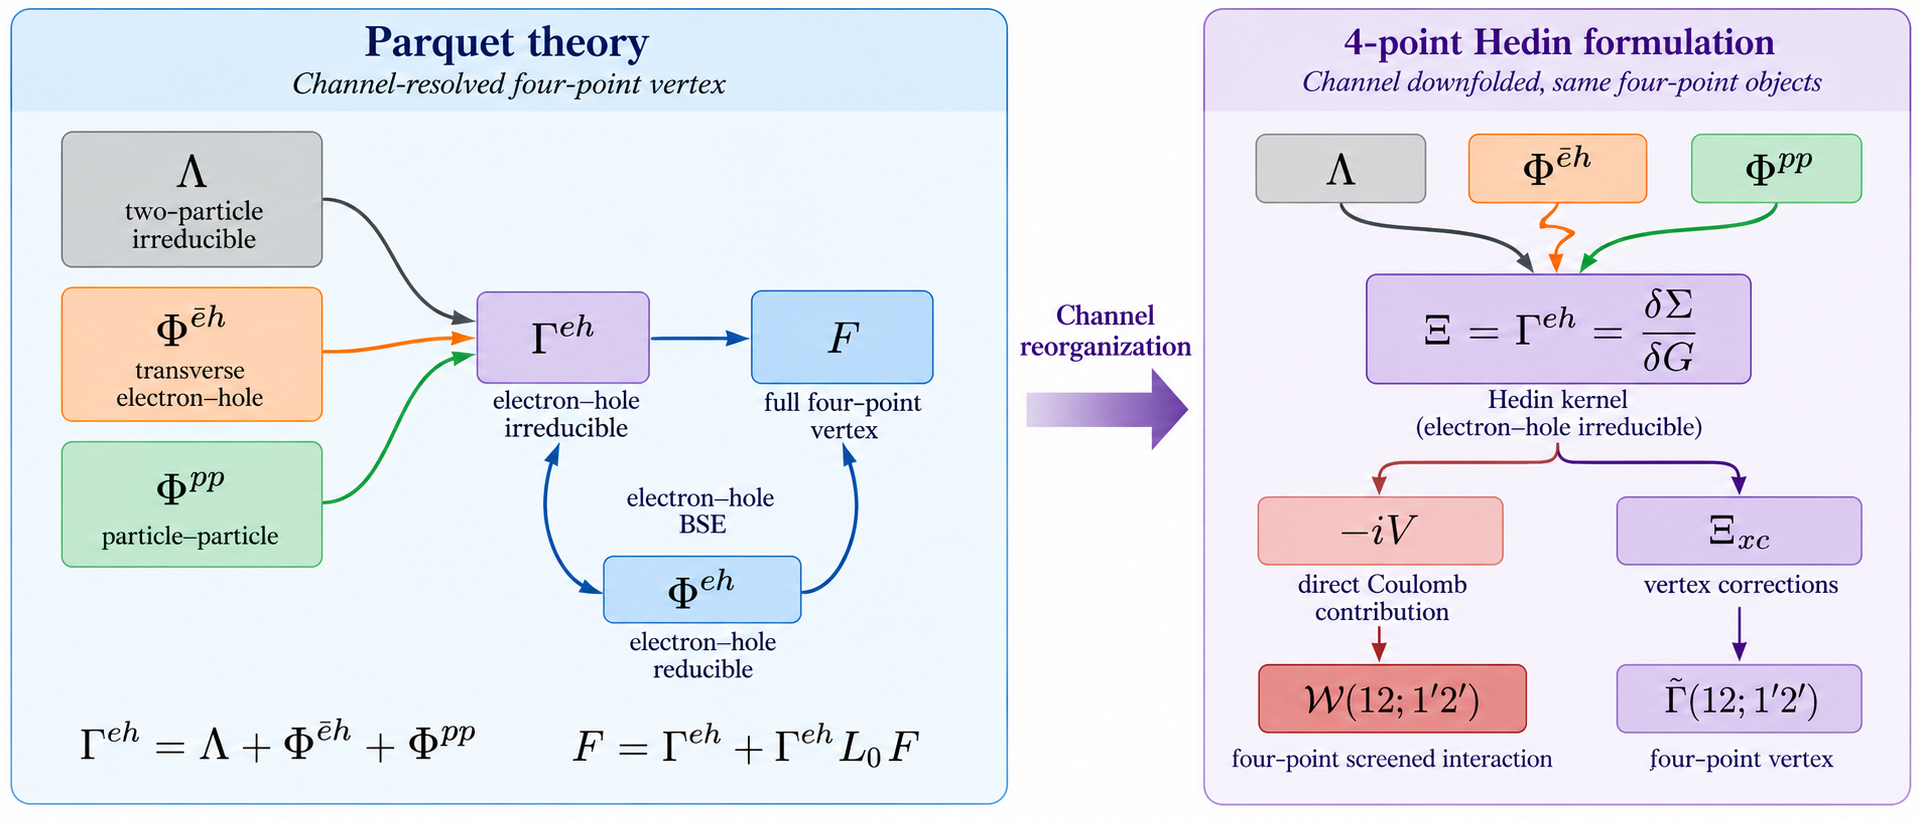
\includegraphics[width=0.7\linewidth]{parquet.png}
\end{center}
\bigskip
\end{abstract}

\maketitle
%%%%%%%%%%%%%%%%%%%%%%%%%
\section{Introduction}
%%%%%%%%%%%%%%%%%%%%%%%%%

Many-body perturbation theory admits several formally exact organizations
of the same underlying many-electron problem.
Among the most prominent are Hedin's equations and the parquet equations.\cite{Hedin1965,DeDominicis_1964b,Bickers_2004}
Although both formulations ultimately describe the same one- and
two-particle correlation functions, they organize the underlying
two-particle information rather differently.

The standard Hedin equations are built around the one-particle Green's
function $G$, the self-energy $\Sigma$, the screened Coulomb interaction
$W$, the irreducible polarizability $P$, and a 3-point vertex.\cite{Hedin1965,MarieAmmarLoos2024}
Their central 4-point kernel is the functional derivative
$\Xi=\delta\Sigma/\delta G$, which is, in general, a three-frequency
object.

Parquet theory instead resolves the full 4-point vertex $F$ according to
two-particle reducibility in the electron-hole ($\eh$), transverse
electron-hole ($\teh$), and particle-particle ($\pp$) channels.\cite{DeDominicis_1964b,Eckhardt2023,MarieLoos2025}
Introducing the fully two-particle-irreducible vertex $\Lambda$ and the
three channel-reducible vertices $\Phi^\eh$, $\Phi^{\teh}$, and
$\Phi^\pp$, the vertex irreducible in the $\eh$ channel contains
$\Lambda$ together with the complete $\teh$ and $\pp$ contributions.

The main result of these notes is that the exact 4-point Hedin kernel is
precisely this $\eh$-irreducible parquet vertex.
Thus parquet keeps the different scattering channels explicit, whereas
the 4-point Hedin formulation combines the channels irreducible with
respect to $\eh$ propagation into a single kernel.

The purpose of these notes is to establish this connection algebraically.
We first derive the 4-point Hedin response equation directly from the
$\eh$ Bethe--Salpeter equation and then discuss how the resulting
channel-centered description relates to the conventional Hedin
organization.
For completeness, we also consider the analogous construction in the
$\pp$ channel, where repeated pair scattering is described by the
4-point $T$ matrix.

%%%%%%%%%%%%%%%%%%%%%%%%%
\section{One- and two-particle quantities}
\label{sec:quantities}
%%%%%%%%%%%%%%%%%%%%%%%%%

Throughout these notes, numerical labels denote collective
space-spin-time variables,
\begin{equation}
	1 \equiv (\bx_1,t_1)
	= (\br_1,\sigma_1,t_1)
\end{equation}
and integration over repeated labels is implied.

%%%%%%%%%%%%%%%%%%%%%%%%%
\subsection{One-particle Green's function}
%%%%%%%%%%%%%%%%%%%%%%%%%

The time-ordered one-particle Green's function is defined as
\begin{equation}
	G(11')
	=
	-\ii
	\mel{
		\Psi_0^N
		}{
		\hat{T}
		[
			\hat{\psi}(1)
			\hat{\psi}^{\dagger}(1')
		]
		}{
		\Psi_0^N
	}
	\label{eq:G_def}
\end{equation}
where $\ket*{\Psi_0^N}$ is the exact $N$-electron ground state and
$\hat{T}$ is the time-ordering operator.

The interacting Green's function satisfies the Dyson equation
\begin{equation}
	G(11')
	=
	G_0(11')
	+
	G_0(12)
	\Sigma(22')
	G(2'1')
	\label{eq:Dyson}
\end{equation}
where $G_0$ is the non-interacting Green's function and $\Sigma$ is
the one-particle irreducible self-energy.

The Dyson equation provides the first example of a recurring idea in
many-body theory: reducible contributions are generated by iterating
an irreducible kernel.
The same principle will appear at the two-particle level through the
Bethe--Salpeter and parquet equations.

%%%%%%%%%%%%%%%%%%%%%%%%%
\subsection{Two-particle Green's function and full vertex}
%%%%%%%%%%%%%%%%%%%%%%%%%

The time-ordered two-particle Green's function is
\begin{equation}
	\begin{split}
	G_2(12;1'2')
	=
	(-\ii)^2
	\mel{
		\Psi_0^N
		}{
		\hat{T}
		[
			\hat{\psi}(1)
			\hat{\psi}(2)
			\hat{\psi}^{\dagger}(2')
			\hat{\psi}^{\dagger}(1')
		]
		}{
		\Psi_0^N
	}
	\end{split}
	\label{eq:G2_def}
\end{equation}

The full two-particle vertex $F$ is defined by amputating the
connected part of $G_2$.
With the conventions adopted here,
\begin{multline}
	G_2(12;34)
	=
	G(13)G(24)
	-
	G(14)G(23)
	\\
	-
	G(11')
	G(3'3)
	F(1'2';3'4')
	G(4'4)
	G(22')
	\label{eq:G2_F}
\end{multline}
The first two terms correspond to the two possible independent
propagations of a pair of fermions, while $F$ contains all connected
two-particle scattering processes.

Fermionic antisymmetry implies the crossing relations
\begin{equation}
	\begin{split}
	F(12;34)
	&=
	-F(21;34)
	\\
	&=
	-F(12;43)
	\\
	&=
	+F(21;43)
	\end{split}
	\label{eq:F_crossing}
\end{equation}
These relations will play an important role when connecting the two
$\eh$ channels.

For a time-independent Hamiltonian, time-translation invariance removes
one overall time variable from a 4-point quantity.
Consequently, the full vertex $F$ depends on three independent time
differences or, equivalently, three independent frequencies.
Different choices of these frequency variables are naturally adapted to
the different parquet channels.

%%%%%%%%%%%%%%%%%%%%%%%%%
\subsection{Electron-hole correlation function}
%%%%%%%%%%%%%%%%%%%%%%%%%

For the connection with Hedin's equations, it is convenient to introduce
the $\eh$ correlation function
\begin{equation}
	L(12;1'2')
	=
	G(11')G(22')
	-
	G_2(12;1'2')
	\label{eq:L_def}
\end{equation}
Its independent-propagation contribution is
\begin{equation}
	L_0(12;1'2')
	=
	G(12')G(21')
	\label{eq:L0_def}
\end{equation}
Substituting Eq.~\eqref{eq:G2_F} into Eq.~\eqref{eq:L_def} gives
\begin{multline}
	L(12;1'2')
	=
	L_0(12;1'2')
	\\
	+
	G(13)
	G(3'1')
	F(34;3'4')
	G(4'2')
	G(24)
	\label{eq:L_F_explicit}
\end{multline}
Using Eq.~\eqref{eq:L0_def}, the same relation reads
\begin{multline}
	L(12;1'2')
	=
	L_0(12;1'2')
	\\
	+
	L_0(13';1'3)
	F(34;3'4')
	L_0(4'2;42')
	\label{eq:L_F}
\end{multline}

Equation~\eqref{eq:L_F}, symbolically $L=L_0+L_0FL_0$, establishes the
direct relation between the full 4-point vertex and the $\eh$ response.

%%%%%%%%%%%%%%%%%%%%%%%%%
\section{Two-particle reducibility and parquet equations}
\label{sec:parquet}
%%%%%%%%%%%%%%%%%%%%%%%%%

In contrast to the one-particle case, where reducibility is associated
with cutting a single propagator line, a 4-point diagram may become
disconnected by cutting two propagator lines.
For a number-conserving fermionic system, there are three topologically
distinct ways of performing such a cut.
They define the electron-hole ($\eh$), transverse electron-hole
($\teh$), and particle-particle ($\pp$) channels.

A connected 4-point diagram is said to be \emph{reducible} in a given
channel if it can be separated into two disconnected pieces by cutting
the corresponding pair of one-particle propagators.
Otherwise, it is irreducible in that channel.
A diagram that is irreducible in all three channels is said to be
\emph{fully two-particle irreducible}.

For a number-conserving theory, a two-particle-reducible diagram belongs
to one and only one of the three channels.
The full vertex therefore admits the exact decomposition
\begin{multline}
	F(12;34)
	=
	\Lambda(12;34)
	+
	\Phi^\eh(12;34)
	\\
	+
	\Phi^{\teh}(12;34)
	+
	\Phi^\pp(12;34)
	\label{eq:parquet_decomposition}
\end{multline}
where $\Lambda$ is the fully two-particle-irreducible vertex and
$\Phi^\eh$, $\Phi^{\teh}$, and $\Phi^\pp$ collect all
diagrams reducible in the corresponding channel.

%%%%%%%%%%%%%%%%%%%%%%%%%
\subsection{Channel-irreducible vertices}
%%%%%%%%%%%%%%%%%%%%%%%%%

It is useful to introduce vertices that are irreducible in one specific
channel but may be reducible in the other two.
For the $\eh$ channel,
\begin{equation}
	\Gamma^\eh(12;34)
	=
	\Lambda(12;34)
	+
	\Phi^{\teh}(12;34)
	+
	\Phi^\pp(12;34)
	\label{eq:Gamma_eh}
\end{equation}
Similarly,
\begin{equation}
	\Gamma^{\teh}(12;34)
	=
	\Lambda(12;34)
	+
	\Phi^\eh(12;34)
	+
	\Phi^\pp(12;34)
	\label{eq:Gamma_ehbar}
\end{equation}
and
\begin{equation}
	\Gamma^\pp(12;34)
	=
	\Lambda(12;34)
	+
	\Phi^\eh(12;34)
	+
	\Phi^{\teh}(12;34)
	\label{eq:Gamma_pp}
\end{equation}

Equivalently, $F=\Gamma^r+\Phi^r$ in each of the three channels.
This identity is particularly important for what follows.
Choosing one of the three channels does not amount to neglecting the
other two.
For example, $\Gamma^\eh$ already contains the complete
$\teh$ and $\pp$ contributions through
Eq.~\eqref{eq:Gamma_eh}.
The distinction between the three formulations is therefore a distinction
in how the two-particle information is organized rather than in the
information retained.

%%%%%%%%%%%%%%%%%%%%%%%%%
\subsection{Bethe--Salpeter equations}
%%%%%%%%%%%%%%%%%%%%%%%%%

The reducible contribution in each channel can be generated by iterating
the corresponding channel-irreducible vertex.
This leads to three Bethe--Salpeter equations for the same full vertex
$F$.

In the $\eh$ channel,
\begin{multline}
	F(12;34)
	=
	\Gamma^\eh(12;34)
	\\
	+
	\Gamma^\eh(13';31')
	G(1'4')
	G(2'3')
	F(4'2;2'4)
	\label{eq:BSE_eh}
\end{multline}
The second term is, by construction, the contribution reducible in the $\eh$ channel.

In the $\teh$ channel,
\begin{multline}
	F(12;34)
	=
	\Gamma^{\teh}(12;34)
	\\
	-
	\Gamma^{\teh}(3'2;32')
	G(1'3')
	G(2'4')
	F(14';1'4)
	\label{eq:BSE_ehbar}
\end{multline}
The minus sign follows from fermionic crossing.


Finally, the $\pp$ BSE reads
\begin{multline}
	F(12;34)
	=
	\Gamma^\pp(12;34)
	\\
	-
	\frac{1}{2}
	\Gamma^\pp(12;1'2')
	G(1'3')
	G(2'4')
	F(3'4';34)
	\label{eq:BSE_pp}
\end{multline}
The factor $1/2$ originates from the antisymmetry of the two-fermion
pair space and avoids double counting equivalent $\pp$
configurations.

Equations~\eqref{eq:BSE_eh}--\eqref{eq:BSE_pp}, together with
Eqs.~\eqref{eq:Gamma_eh}--\eqref{eq:Gamma_pp}, form the two-particle
core of the parquet equations.
Each BSE resums diagrams reducible in one particular channel, while its
irreducible kernel contains the fully irreducible vertex and the
contributions reducible in the other two channels.

%%%%%%%%%%%%%%%%%%%%%%%%%
\subsection{Crossing relations}
%%%%%%%%%%%%%%%%%%%%%%%%%

The three channel equations are not independent.
Their mutual consistency is enforced by fermionic crossing symmetry.
While the $\pp$-irreducible vertex possesses the same antisymmetry as the
full vertex, the two $\eh$ irreducible vertices are related to
one another through
\begin{align}
	\Gamma^\eh(21;34)
	& =
	-
	\Gamma^{\teh}(12;34)
	\label{eq:Gamma_crossing_1}
	\\
	\Gamma^\eh(12;43)
	& =
	-
	\Gamma^{\teh}(12;34)
	\label{eq:Gamma_crossing_2}
\end{align}

Consequently, the three BSEs should not be viewed as three independent
descriptions of different physical systems.
They are three channel-resolved representations of the same full
4-point vertex.
Their simultaneous solution makes the different two-particle scattering
processes explicit while avoiding double counting between the channels.

This observation will be central in the following section.
In particular, selecting the $\eh$ Bethe--Salpeter equation while retaining
the exact kernel $\Gamma^\eh$ does not discard either the
$\teh$ or the $\pp$ channel.
Rather, according to Eq.~\eqref{eq:Gamma_eh}, these two channels are
already contained in the $\eh$-irreducible kernel.
This provides the starting point for the connection between parquet theory
and the 4-point Hedin equations.\cite{StarkeKresse2012,OrlandoRomanielloLoos2023}

%%%%%%%%%%%%%%%%%%%%%%%%%
\section{Closing the parquet equations}
\label{sec:closing_parquet}
%%%%%%%%%%%%%%%%%%%%%%%%%

The parquet equations determine the full two-particle vertex once the
fully irreducible vertex $\Lambda$ and the one-particle Green's function
are known.
To obtain a closed many-body theory, the two-particle vertex must in turn
be connected to the one-particle self-energy.

This connection follows from the equation of motion for the one-particle
Green's function.\cite{MarieLoos2025}
It yields the exact Dyson--Schwinger equation
\begin{equation}
	\Sigma(11')
	=
	-\ii
	v(12;3'2')
	G_2(3'2';32)
	G^{-1}(31')
	\label{eq:SDE_G2}
\end{equation}
where $v$ is the bare Coulomb interaction.

Using the decomposition of the two-particle Green's function in terms of
the full vertex $F$, Eq.~\eqref{eq:G2_F}, one obtains
\begin{multline}
	\Sigma(11')
	=
	\Sigma_{\Hx}(11')
	\\
	-
	\ii
	v(12;3'2')
	G(3'3)
	G(4'2)
	G(2'4)
	F(34;4'1')
	\label{eq:SDE_F}
\end{multline}
Here $\Sigma_{\Hx}$ denotes the Hartree-exchange self-energy and the
second term is the exact correlation self-energy.
The Schwinger--Dyson equation therefore closes the one- and two-particle
levels: the full vertex feeds back into the one-particle propagator through
the self-energy, while the Dyson equation determines $G$ from $\Sigma$.
Together with the parquet decomposition and the three Bethe--Salpeter
equations, these relations form a closed self-consistent hierarchy once
the fully irreducible vertex $\Lambda$ is specified.

The fully irreducible vertex $\Lambda$ is the only quantity in this set
that is not determined by the parquet equations themselves.
At the exact level it contains all diagrams that are irreducible in each
of the three two-particle channels.

A frequently employed closure is the \emph{parquet approximation}, in
which $\Lambda$ is replaced by the antisymmetrized bare interaction,
\begin{equation}
	\Lambda(12;1'2')
	\approx
	-\ii \bar v(12;1'2')
	=
	-\ii
	\left[
		v(12;1'2')
		-
		v(12;2'1')
	\right]
	\label{eq:parquet_approximation}
\end{equation}
This approximation will not be required in the following derivation:
the connection with Hedin's equations is established at the exact level.


%%%%%%%%%%%%%%%%%%%%%%%%%
\section{From parquet to the 4-point Hedin equation}
\label{sec:parquet_to_hedin4}
%%%%%%%%%%%%%%%%%%%%%%%%%

We now establish the central connection between parquet theory and the
4-point formulation of Hedin's equations.

%%%%%%%%%%%%%%%%%%%%%%%%%
\subsection{Attaching the external propagators}
%%%%%%%%%%%%%%%%%%%%%%%%%

Substituting the $\eh$ Bethe--Salpeter equation,
Eq.~\eqref{eq:BSE_eh}, into Eq.~\eqref{eq:L_F} and collecting the
external propagators gives, in symbolic notation,
\begin{equation}
\begin{split}
	L
	&=
	L_0
	+
	L_0\left(\Gamma^\eh+\Gamma^\eh L_0F\right)L_0
	\\
	&=
	L_0
	+
	L_0\Gamma^\eh\left(L_0+L_0FL_0\right)
	\\
	&=
	L_0
	+
	L_0\Gamma^\eh L
\end{split}
	\label{eq:L_BSE_Gammaeh}
\end{equation}
No approximation is involved.
Attaching the external one-particle propagators to the $\eh$ parquet BSE
therefore converts it directly into a 4-point Bethe--Salpeter equation
for the response.
Conversely, amputating the external propagators recovers the original
$\eh$ BSE.

%%%%%%%%%%%%%%%%%%%%%%%%%
\subsection{Identification of the Hedin kernel}
%%%%%%%%%%%%%%%%%%%%%%%%%

In the 4-point formulation of Hedin's equations, the same response
satisfies
\begin{equation}
	L
	=
	L_0
	+
	L_0\Xi L
	\label{eq:Hedin4_response}
\end{equation}
with
\begin{equation}
	\Xi(12;1'2')
	=
	\frac{\delta\Sigma(11')}{\delta G(2'2)}
	\label{eq:Xi_def}
\end{equation}
Comparison with Eq.~\eqref{eq:L_BSE_Gammaeh} gives the exact identity
\begin{equation}
	\Xi(12;1'2')
	=
	\frac{\delta\Sigma(11')}{\delta G(2'2)}
	=
	\Gamma^\eh(12;1'2')
	\label{eq:central_identity}
\end{equation}

Equation~\eqref{eq:central_identity} is the central result of these notes.
Together with Eq.~\eqref{eq:Gamma_eh}, it shows that the Hedin kernel is
irreducible in the $\eh$ channel while containing the fully irreducible
vertex and all contributions reducible in the $\teh$ and $\pp$ channels.
Selecting the $\eh$ response channel therefore does not discard the
other two channels; it incorporates them into the $\eh$-irreducible
kernel.

This gives a precise meaning to channel downfolding.
Parquet retains $\Lambda$, $\Phi^{\teh}$, and $\Phi^\pp$ as separate
objects determined by coupled channel equations, whereas the 4-point
Hedin formulation combines them into the single three-frequency kernel
$\Xi$.

\section{Parquet as a channel-resolved Hedin theory}
\label{sec:interpretation}
%%%%%%%%%%%%%%%%%%%%%%%%%

Equation~\eqref{eq:central_identity} makes the relation between parquet
and Hedin theory particularly transparent.
Parquet is a channel-resolved representation: the $\teh$ and $\pp$
contributions remain explicit and satisfy their own Bethe--Salpeter
equations.
The 4-point Hedin formulation instead uses their sum with $\Lambda$ as
the $\eh$-irreducible kernel $\Xi$.
Calling the latter a downfolded representation is therefore only a
statement about how the same exact information is organized.

%%%%%%%%%%%%%%%%%%%%%%%%%
\subsection{Frequency structure}
%%%%%%%%%%%%%%%%%%%%%%%%%

A general 4-point vertex depends on three independent frequencies.
Each parquet channel has a natural transfer frequency, so the same
4-point object may be parametrized in terms of
$(\nu,\nu',\omega_\eh)$, $(\nu,\nu',\omega_{\teh})$, or
$(\nu,\nu',\omega_\pp)$ depending on the channel under consideration.
Parquet makes these channel-adapted structures explicit.

In the Hedin organization, the $\teh$ and $\pp$ contributions are instead
encoded in the full three-frequency dependence of the kernel.
When the direct Coulomb contribution is separated, the repeated direct
$\eh$ screening is described by the simpler bosonic quantity
$W(\omega_\eh)$, while the remaining vertex structure resides in
$\Xi_{\xc}(\nu,\nu',\omega_\eh)$.

%%%%%%%%%%%%%%%%%%%%%%%%%
\subsection{Explicit and implicit channel coupling}
%%%%%%%%%%%%%%%%%%%%%%%%%

For a fixed channel-irreducible vertex, each parquet Bethe--Salpeter
equation is linear in the full vertex.
The complete parquet problem is nevertheless nonlinear because the
irreducible vertex in one channel depends on contributions reducible in
the other channels.
Its nonlinearity therefore appears as an explicit feedback between
coupled channel equations.

Hedin theory packages the same feedback into the functional dependence of
the kernel on the Green's function.
It is consequently more compact, but the channel coupling is less
explicit.
This should not be interpreted as a difference in the formal degree of
nonlinearity of the exact theories; the same information is distributed
differently among their basic variables.
The passage from parquet to the 4-point Hedin formulation is thus a
channel reorganization.

\section{Particle-particle analogue}
\label{sec:pp_analogue}
%%%%%%%%%%%%%%%%%%%%%%%%%

The same channel-centered construction can be carried out in the $\pp$
sector.\cite{MarieRomanielloLoos2024,MarieRomanielloBlaseLoos2025}
Starting from the $\pp$ parquet BSE, Eq.~\eqref{eq:BSE_pp}, the pair
propagator obeys
\begin{multline}
	K(12;1'2')
	=
	K_0(12;1'2')
	\\
	-
	\frac{1}{2}
	K(12;44')
	\Gamma^\pp(44';33')
	K_0(33';1'2')
	\label{eq:K_parquet}
\end{multline}
with
\begin{equation}
	K_0(12;1'2')
	=
	\frac{1}{2}
	\left[
		G(11')G(22')
		-
		G(21')G(12')
	\right]
	\label{eq:K0_def}
\end{equation}
The factor $1/2$ reflects the normalization of the antisymmetric pair
space.

The same response follows from an anomalous functional derivative,
\begin{equation}
	K
	=
	K_0
	-
	K\Xi^\pp K_0
	\label{eq:K_pp_Hedin}
\end{equation}
where
\begin{equation}
	\Xi^\pp(12;1'2')
	=
	\eval{
	\fdv{\Sigma^{\ee}(1'2')}{G^{\ee}(12)}
	}_{U=0}
	\label{eq:Xi_pp_def}
\end{equation}
Comparison of the two equations yields
\begin{equation}
	2\Xi^\pp
	=
	\Gamma^\pp
	\label{eq:Xi_pp_parquet}
\end{equation}
Together with Eq.~\eqref{eq:Gamma_pp}, this shows that the two electron-hole
channels are downfolded into the $\pp$-irreducible kernel in exactly the
same sense as the $\teh$ and $\pp$ channels are downfolded into
$\Gamma^\eh$ in the conventional Hedin construction.

Repeated pair scattering is naturally collected into a 4-point
$T$ matrix.\cite{MarieRomanielloLoos2024}
At the lowest vertex level this recovers the familiar $T$-matrix
self-energy.
Unlike the ordinary Hedin kernel, however, $\Xi^\pp$ is defined through
an anomalous self-energy and anomalous propagator.
A pairing field must therefore be retained during the functional
derivation and the number-conserving limit taken only afterwards.
Beyond the lowest-order vertex approximation, this anomalous
Nambu--Gorkov sector is required to generate $\Xi^\pp$ consistently.

\section{Exact equivalence and approximate closures}
\label{sec:approximations}
%%%%%%%%%%%%%%%%%%%%%%%%%

The relation derived above is exact.\cite{KuglerVonDelft2018}
At the exact level, the $\eh$-irreducible parquet vertex and the
functional Hedin kernel are the same object.
This does not imply, however, that independently truncated parquet and
Hedin constructions remain equivalent.\cite{KuglerVonDelft2018,Baym_1961,Baym_1962}

A Hedin-type closure naturally starts from an approximate self-energy and
defines the corresponding kernel by
\begin{equation}
	\Xi^{\rm app}
	=
	\frac{\delta\Sigma^{\rm app}}{\delta G}
	\label{eq:Hedin_closure}
\end{equation}
A parquet closure instead starts from an approximation to the fully
irreducible vertex, solves the coupled channel equations, and obtains the
self-energy from the resulting full vertex through the
Schwinger--Dyson equation.

For an approximate parquet solution, the $\eh$-irreducible vertex is
\begin{equation}
	\Gamma^\eh_{\rm P}
	=
	\Lambda^{\rm app}
	+
	\Phi^{\teh}_{\rm app}
	+
	\Phi^\pp_{\rm app}
	\label{eq:Gamma_parquet_approx}
\end{equation}
whereas differentiating the corresponding parquet self-energy gives
\begin{equation}
	\Xi_{\rm FD}
	=
	\frac{\delta\Sigma^{\rm app}_{\rm P}}{\delta G}
	\label{eq:Xi_functional_derivative}
\end{equation}
In general,
\begin{equation}
	\Xi_{\rm FD}
	\neq
	\Gamma^\eh_{\rm P}
	\label{eq:approx_mismatch}
\end{equation}
because the functional derivative acts on every explicit and implicit
Green's function contained in the approximate self-energy.
Truncation and functional differentiation therefore do not generally
commute.

The parquet approximation of Eq.~\eqref{eq:parquet_approximation} provides a
particularly simple illustration.
The Schwinger--Dyson self-energy constructed from the parquet vertex is
consistent with that vertex by construction, but its functional
derivative generates a different two-particle kernel in general.\cite{KuglerVonDelft2018}
Thus the exact statement that parquet is a channel-resolved version of
Hedin theory should not be interpreted as a one-to-one correspondence
between arbitrary finite approximations in the two formalisms.

%%%%%%%%%%%%%%%%%%%%%%%%
\bibliography{parquet-mr-hedin}
%%%%%%%%%%%%%%%%%%%%%%%%

\end{document}

